%
% main.tex -- Paper zum Thema Audio-Kompression mit Daubechies-Wavelets
%
% (c) 2019 Hochschule Rapperswil
%
\chapter{Audio-Komprimierung mit Daubechies Wavelets\label{chapter:compress}}
\lhead{Audio-Komprimierung mit Daubechies Wavelets}
\begin{refsection}
\chapterauthor{Julian Bärtschi}

\section{Audio-Komprimierung}
\rhead{Vorwort}
Die Menge an produzierten Daten nimmt jährlich rasant zu.
Immer höher aufgelöste Bild-, Video- und Audiodaten spielen dabei eine zentrale Rolle.
Um den Berg an Daten im Griff zu behalten, ist Datenkomprimierung (lat.~comprimere, `zusammendrücken') unerlässlich. 

Das Ziel der Datenkomprimierung ist es, die vorhandenen Daten so zu verdichten, dass der Speicherbedarf möglichst reduziert werden kann.
Es sollen für die Speicherung, wie auch für die Übertragung der Daten möglichst wenig Ressourcen benötigt werden.

Diese Arbeit wird auf Audiodaten beschränkt.
Dabei ist das Ziel nicht etwa die Entwicklung eines Kompressionsalgorithmus sondern das Aufzeigen von Möglichkeiten der Komprimierung mit Hilfe von Wavelets.
Des Weiteren steht eine exakte Rekonstruktion nicht im Vordergrund, jedoch soll für den Hörer möglichst keinen Unterschied zum Original wahrnehmbar sein.

\subsection{Verlustfreie Komprimierung}
Bei der verlustfreien Komprimierung wird gewährleistet, dass die Originaldaten exakt aus den komprimierten Daten wiederhergestellt werden können.
Es wird die Tatsache ausgenutzt, dass gewisse Daten redundant vorkommen. 
Deshalb spricht man auch von Redundanzreduktion.

Verlustfreie Komprimierung findet breite Anwendung.
Insbesondere bei Datenarchivierung sollen die Originaldaten exakt erhalten bleiben und darum wird häufig eine solche Kompressionstechnik verwendet.
Namhafte Beispiele von verlustfreier Komprimierung sind beispielsweise das ZIP-Dateiformat, die Portable Network Graphics (PNG) oder im Bezug auf Audiodaten der Free Lossless Audio Codec (FLAC).
Beispielsweise kann mit dem FLAC-8 der Speicherplatzbedarf auf unter 66 Prozent der Originaldatei reduziert werden, ohne dabei Informationen zu verlieren.\cite{wikipedia:flac}

\subsection{Verlustbehaftete Komprimierung}
Bei der verlustbehafteten Komprimierung soll nur der nötige Teil der Originaldaten erhalten bleiben.
Somit ist es möglich, den benötigten Speicherplatz auf ein Minimum zu reduzieren.
Das hat jedoch zur Folge, dass die Originaldaten nicht mehr exakt wiederhergestellt werden können. 
Somit ist sie nicht mehr umkehrbar.
Man kann unnötige Daten entfernen und somit die Datenmenge reduzieren.
Deshalb spricht man auch von Irrelevanzreduktion.
Um zu entscheiden, welche Teile wichtig und welche entbehrlich sind, wird auf die menschliche Wahrnehmung geachtet.
Die verlustbehaftete Komprimierung wird insbesondere für Multimedia-Daten häufig verwendent.
Weil die menschliche Sinneswahrnehmung nicht alle Frequenzen und Töne gleich gut aufnimmt, können gewisse Bereiche weggelassen werden.
Mehr dazu im nächsten Kapitel.

Mit der verlustbehafteten Kompression können sehr hohe Kompressionsraten erreicht werden, welche aber stets mit einer Qualitätseinbusse kommen.
Diesen Abtausch von hoher Kompression mit schlechter Qualität gilt es abzuschätzen.

\section{Psychoakustik}
\rhead{Psychoakustik}
Das menschliche Gehör verarbeitet Schallwellen nicht einfach wie ein Mikrofon.
Um ein Schallereignis zu beurteilen haben Psychoakustiker eine Vielzahl an Parametern identifiziert, beispielsweise Lautheit und Schärfe, auf welche in dieser Arbeit aber nicht weiter eingegangen wird.

\begin{figure}
	\centering
	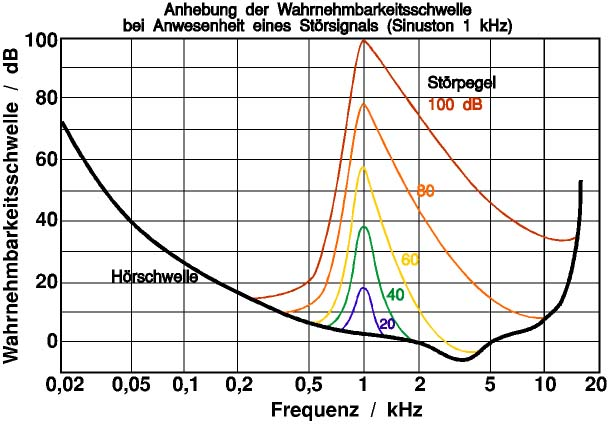
\includegraphics[width=0.6\linewidth]{papers/compress/Bilder/Akustik_Mithoerschwelle2}
	\caption{Wahrnehmbarkeit von Schallsignalen bei Anwesenheit von Störsignalen \cite{skript:Akustik2}}
	\label{fig:Wahrnehmbarkeitsschwelle}
\end{figure}

In \autoref{fig:Wahrnehmbarkeitsschwelle} dargestellt ist ein Modell der Wahrnehmbarkeitsschwelle des menschlichen Gehörs.
Bei einem vorhandenen Störsignal, hier $1\,\text{kHz}$, wird diese Schwelle merklich angehoben.
Auch zeitlich werden leise Töne kurz vor und nach einem lauten Ton verdeckt.\cite{wikipedia:Psychoakustik}

Nun folgt die Überlegung, dass jene Daten die nicht wahrnehmbar sind (unter der Schwelle) redundant sind und weggelassen werden können.
Dies suggeriert grosses Potential für die verlustbehaftete Komprimierung.

\section{Warum Daubechies-Wavelets?}
\rhead{Warum Daubechies-Wavelets?}
\label{chapter:daubechies}
Um ein Signal möglichst gut zu analysieren, muss zuerst ein geeignetes Wavelet gewählt werden.
Die in \autoref{chapter:kompakt} vorgestellten Daubechies-Wavelets besitzen sehr nützliche Eigenschaften.
Um die folgenden Abschnitte etwas übersichtlicher zu gestalten wird der Term `Daubechies-Wavelet N-ter Ordnung' nun mit `dbN' abgekürzt.
Das Haar-Wavelet (db1) hat die Eigenschaft, dass es verschwindet, solange nicht mindestens ein lineares Signal analysiert wird.
Für das db2 gilt dasselbe mit quadratischen Funktionen. 
Die Ordnung des Wavelets nimmt also zusammen mit der Ordnung des analysierten Signals zu.
\begin{figure}
	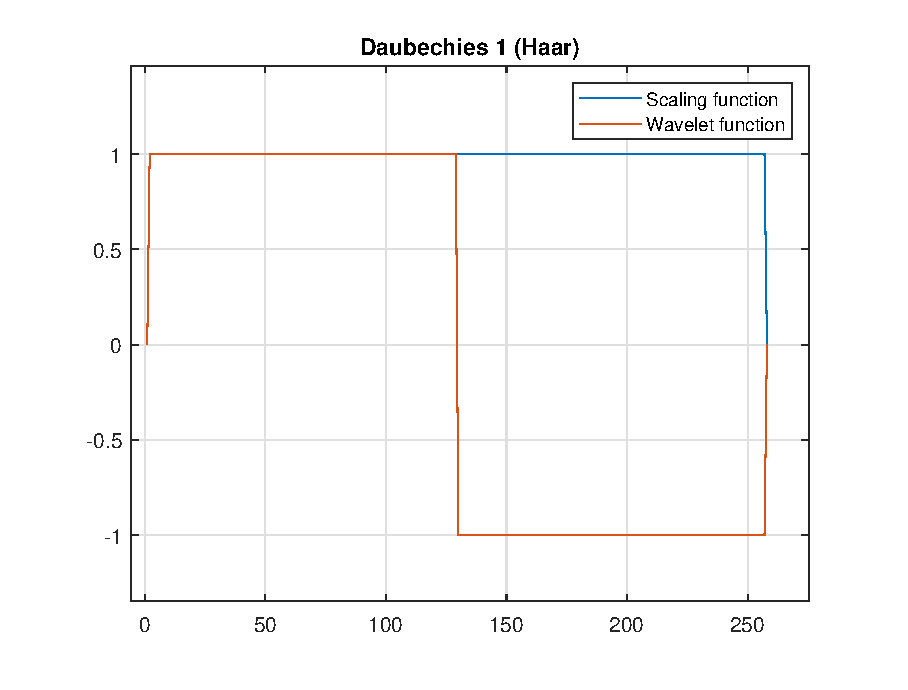
\includegraphics[width=0.5\linewidth]{papers/compress/Bilder/db1}
	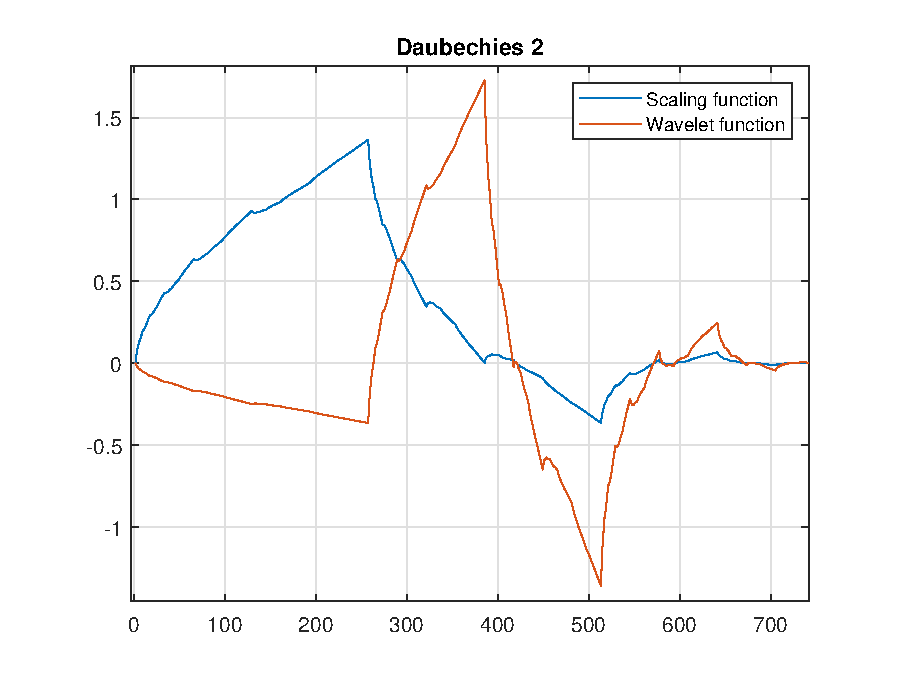
\includegraphics[width=0.5\linewidth]{papers/compress/Bilder/db2}
	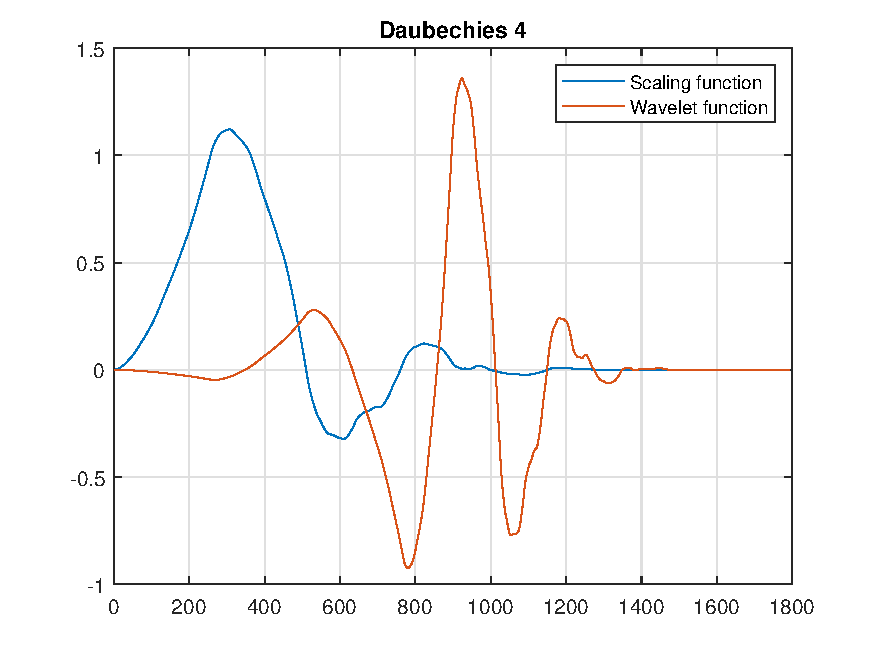
\includegraphics[width=0.5\linewidth]{papers/compress/Bilder/db4}
	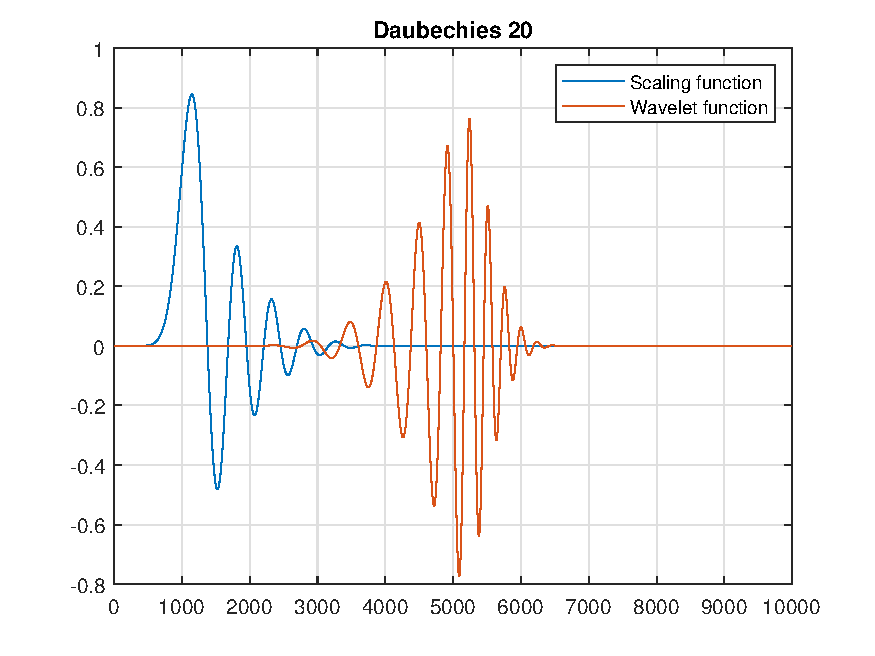
\includegraphics[width=0.5\linewidth]{papers/compress/Bilder/db20}
	\label{fig:dbN}
	\caption{Daubechies-Wavelets unterschiedlicher Ordnungen.}
\end{figure}

Da im Audiobereich sehr transiente Signale möglich sind, können Daubechies-Wavelets einer hohen Ordnung sehr gute Werte liefern.
Das bedeutet zum einen, dass sehr unterschiedliche Signale damit abgetastet werden können und zum anderen, dass die Wavelettransformationen genau Null geben, wenn sie auf Signale der tieferen Ordnung angewendet werden.
Wenn man die Wahrnehmbarkeitsschwelle von \autoref{fig:Wahrnehmbarkeitsschwelle} betrachtet, liegt es nahe, dass eine Folge von Nullwerten oder auch Werte in der Nähe von Null nicht gespeichert werden müssen.
Somit bilden die Daubechies-Wavelets eine gute Grundlage für diese Anwendung.
Für diese Arbeit wurden hauptsächlich die beiden Wavelets `db4' sowie `db20' verwendet.
Experimentell hat sich gezeigt, dass diese sehr gut auf unterschiedlichste Audiodaten passen.

\section{Anwendung}
\rhead{Anwendung}
Für die Analyse von Audiodaten wird eine Multiskalenanalyse, wie in \autoref{chapter:msa} beschrieben, durchgeführt.
Die Anzahl der Levels (\textit{n}) dieser Analyse wird anhand der Länge (\textit{l}) des Signals mit
\begin{equation}
\textit{n} = \log_2{\textit{l}}
\end{equation}
berechnet.

Als Beispiel wird die Analyse einer gewöhnlichen Sägezahnschwingung in \autoref{fig:sawtooth}) dargestellt.
\begin{figure}
	\centering
	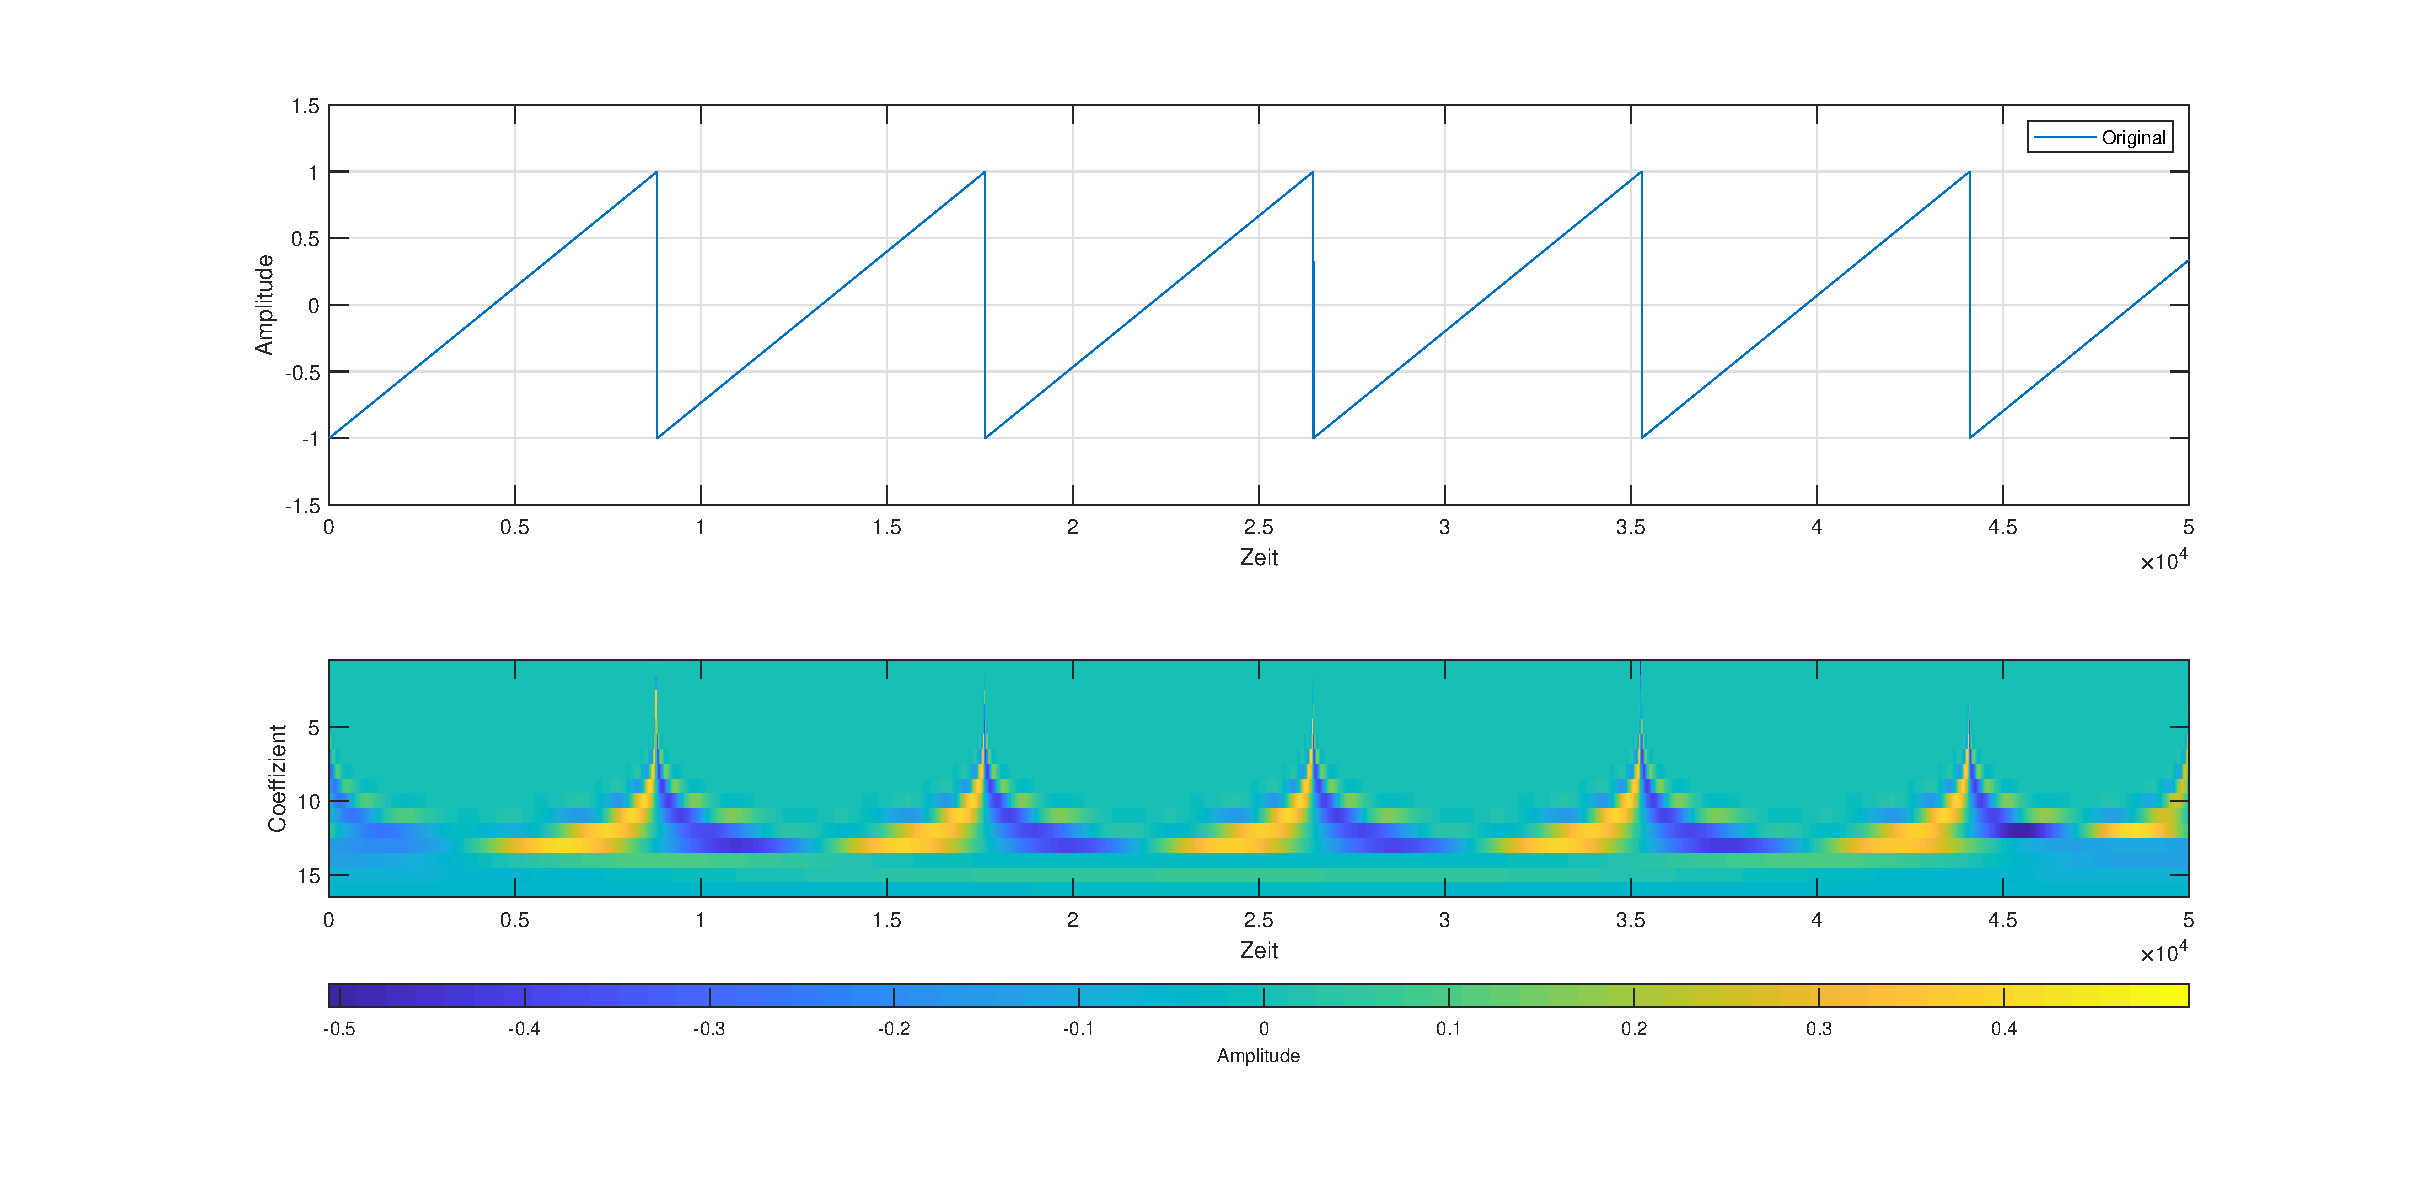
\includegraphics[width=\linewidth]{papers/compress/Bilder/sawtooth}
	\caption{Multiskalenanalyse einer Sägezahnschwingung}
	\label{fig:sawtooth}
\end{figure}
Während dem linearen Anstieg des Sägezahns ist erkennbar, wie die Multiskalenanalyse über alle Skalierungslevels gleich Null ist.
In diesem Beispiel wurde ein db4 verwendet.
Sobald diese unterschiedlich skalierten Wavelets in den transienten Bereich gelangen, ist ein Wert ungleich Null erkennbar.
Für die sehr klein skalierten Wavelets ist das nur in unmittelbarer Umgebung von diesem Sprung der Fall.
Alle anderen Koeffizienten können also komprimiert werden.

Doch wenn nun auch Rauscheffekte gelöscht werden, weil sie nicht stark ins Gewicht fallen, können negative Auswirkungen auf das Hörerlebnis entstehen. 
Koeffizienten, welche nicht stark ins Gewicht fallen, können mit wenigen Bits gespeichert werden, wodurch sie grössere Quantisierungsstufen bilden. 
Dann fehlen sie nicht komplett aber brauchen auch nicht den vollen Speicherplatz.
Nun stellt sich die Frage, ab wann eine solche Quantisierung sinnvoll ist und wann ein Koeffizient ganz weggelassen werden kann. 

\begin{figure}
	\centering
	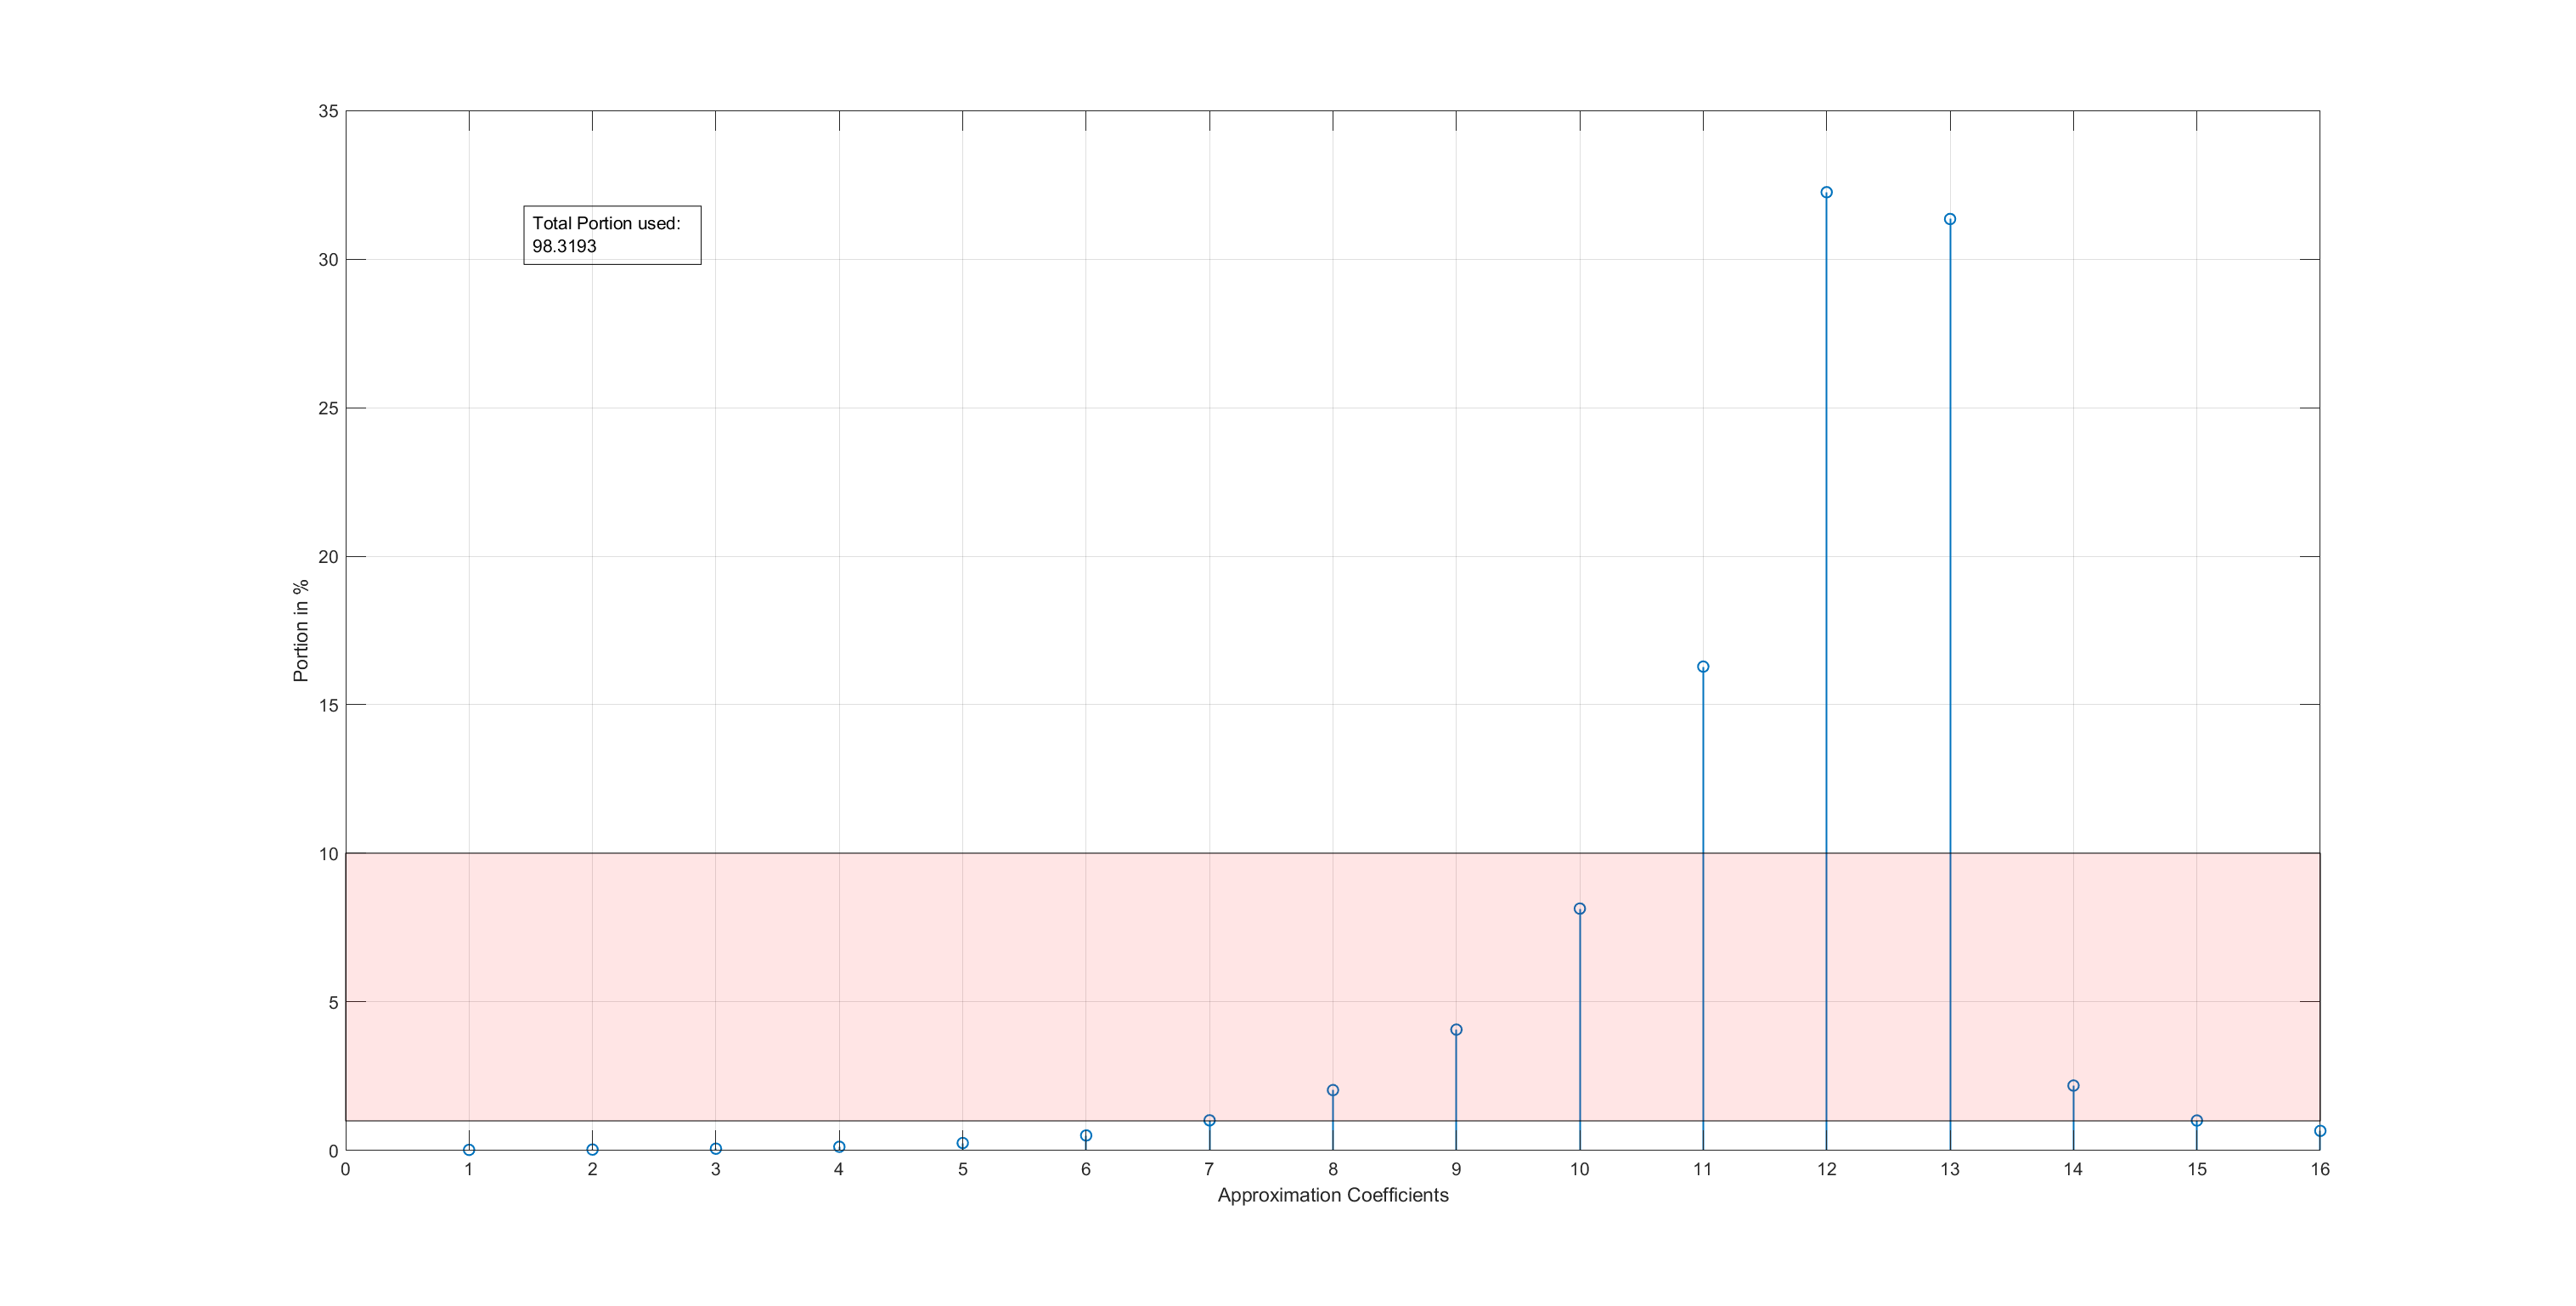
\includegraphics[width=\linewidth]{papers/compress/Bilder/recCoefs}
	\caption{Anteil der einzelnen Levels am gesamten Signal (in Prozent) mit Quantisierungsschranke (rot).}
	\label{fig:coefficients}
\end{figure} 

Wenn anschliessend alle Levels überlagert werden, kann das exakte Signal rekonstruiert werden.
Das Ziel ist jedoch, nur das nötige zu speichern.
Um das zu erreichen muss entschieden werden, ab wann es Sinn macht, die Werte zu speichern oder gegebenenfalls einzusparen.

Für einen ersten Versuch wird der Anteil der einzelnen Levels über das ganze Signal berechnet.
In \autoref{fig:coefficients} ist graphisch dargestellt, welchen Anteil vom originalen Signal die unterschiedlichen Diletationen beinhalten.
Eine ungefähre Grössenanordnung lässt sich für einfache Signale wie in \autoref{fig:sawtooth} auch optisch einschätzen.
Signale mit breiten Bereichen einer hohen Magnitude resultieren auch in einem hohen Anteil. 
Hingegen haben Signale, welche hauptsächlich Magnituden um den Nullpunkt herum besitzen einen eher geringen Einfluss auf das Signal.
Allerdings spielen die Anteile mit kleiner Skalierung insbesondere für Rauscheffekte noch eine Rolle.

Im nächsten Schritt werden zwei Grenzen gesetzt.
Eine obere bei  $10\,\text{\%}$ und eine untere bei $1\,\text{\%}$ der Gesamtsignalstärke.
Diese `Schranke' unterteilt den Graphen nun in drei Bereiche. 
Oberhalb der Schranke sollen die exakten Werte übernommen werden, was beispielsweise einem double-precision floating-point Format mit 64 Bit entspricht.
Unterhalb der Schranke können die Werte jedoch ganz weggelassen werden.
Der Bereich innerhalb der Schranke bildet einen Übergangsbereich.
Die Werte sollen erhalten bleiben jedoch ist die Genauigkeit nicht vordergründig.

Beim Beispiel des Sägezahnes ist in \autoref{fig:coefficients} ersichtlich, dass die Levels 11, 12 und 13 exakt übernommen werden.
Hingegen werden die Levels 1 bis 6 sowie 16 weggelassen und die übrigen quantisiert.
Mit `Total Portion used' wird angegeben welcher Anteil des originalen Signals damit noch wiederhergestellt werden kann.

Der IEEE-754 Standart \cite{article:IEEE-754} beschreibt, wie double-precision floating-point Zahlen gespeichert werden sollen. 
Von den vorhandenen 64 Bit werden 52 für die Mantisse gebraucht.
Für die Quantisierung ist eine solche Genauigkeit überflüssig, da die entsprechende Zahl auf wenigen Nachkommastellen gerundet werden soll.
Wird diese Mantisse nun beispielsweise auf 5 Bit gekürzt kann viel gespart werden.
Von den ursprünglichen 64 Bit bleiben 17 Bit übrig, was noch ungefähr $26.6\,\text{\%}$ des Speicherplatzes entspricht.
Selbstverständlich bedeutet das nicht, dass der gesamte Speicherplatz nur noch knapp einem viertel vom Original entspricht. 
Die tatsächliche Verminderung ist stark signalabhängig.
Es kann somit keine exakte Einschätzung für alle Arten von Audiodaten getroffen werden. 

\subsection{Harmonische Signale}
Als erstes stellt sich die Frage, ob diese Analyse für harmonische Signale interessant ist.
Die Fouriertheorie (\autoref{chapter:fourier}) ermöglicht es einem, harmonische Signale mit relativ wenigen harmonischen Schwingungen zu rekonstruieren.
Doch wie gut funktioniert es mit den hier verwendeten Daubechies-Wavelets?

\begin{figure}
	\centering
	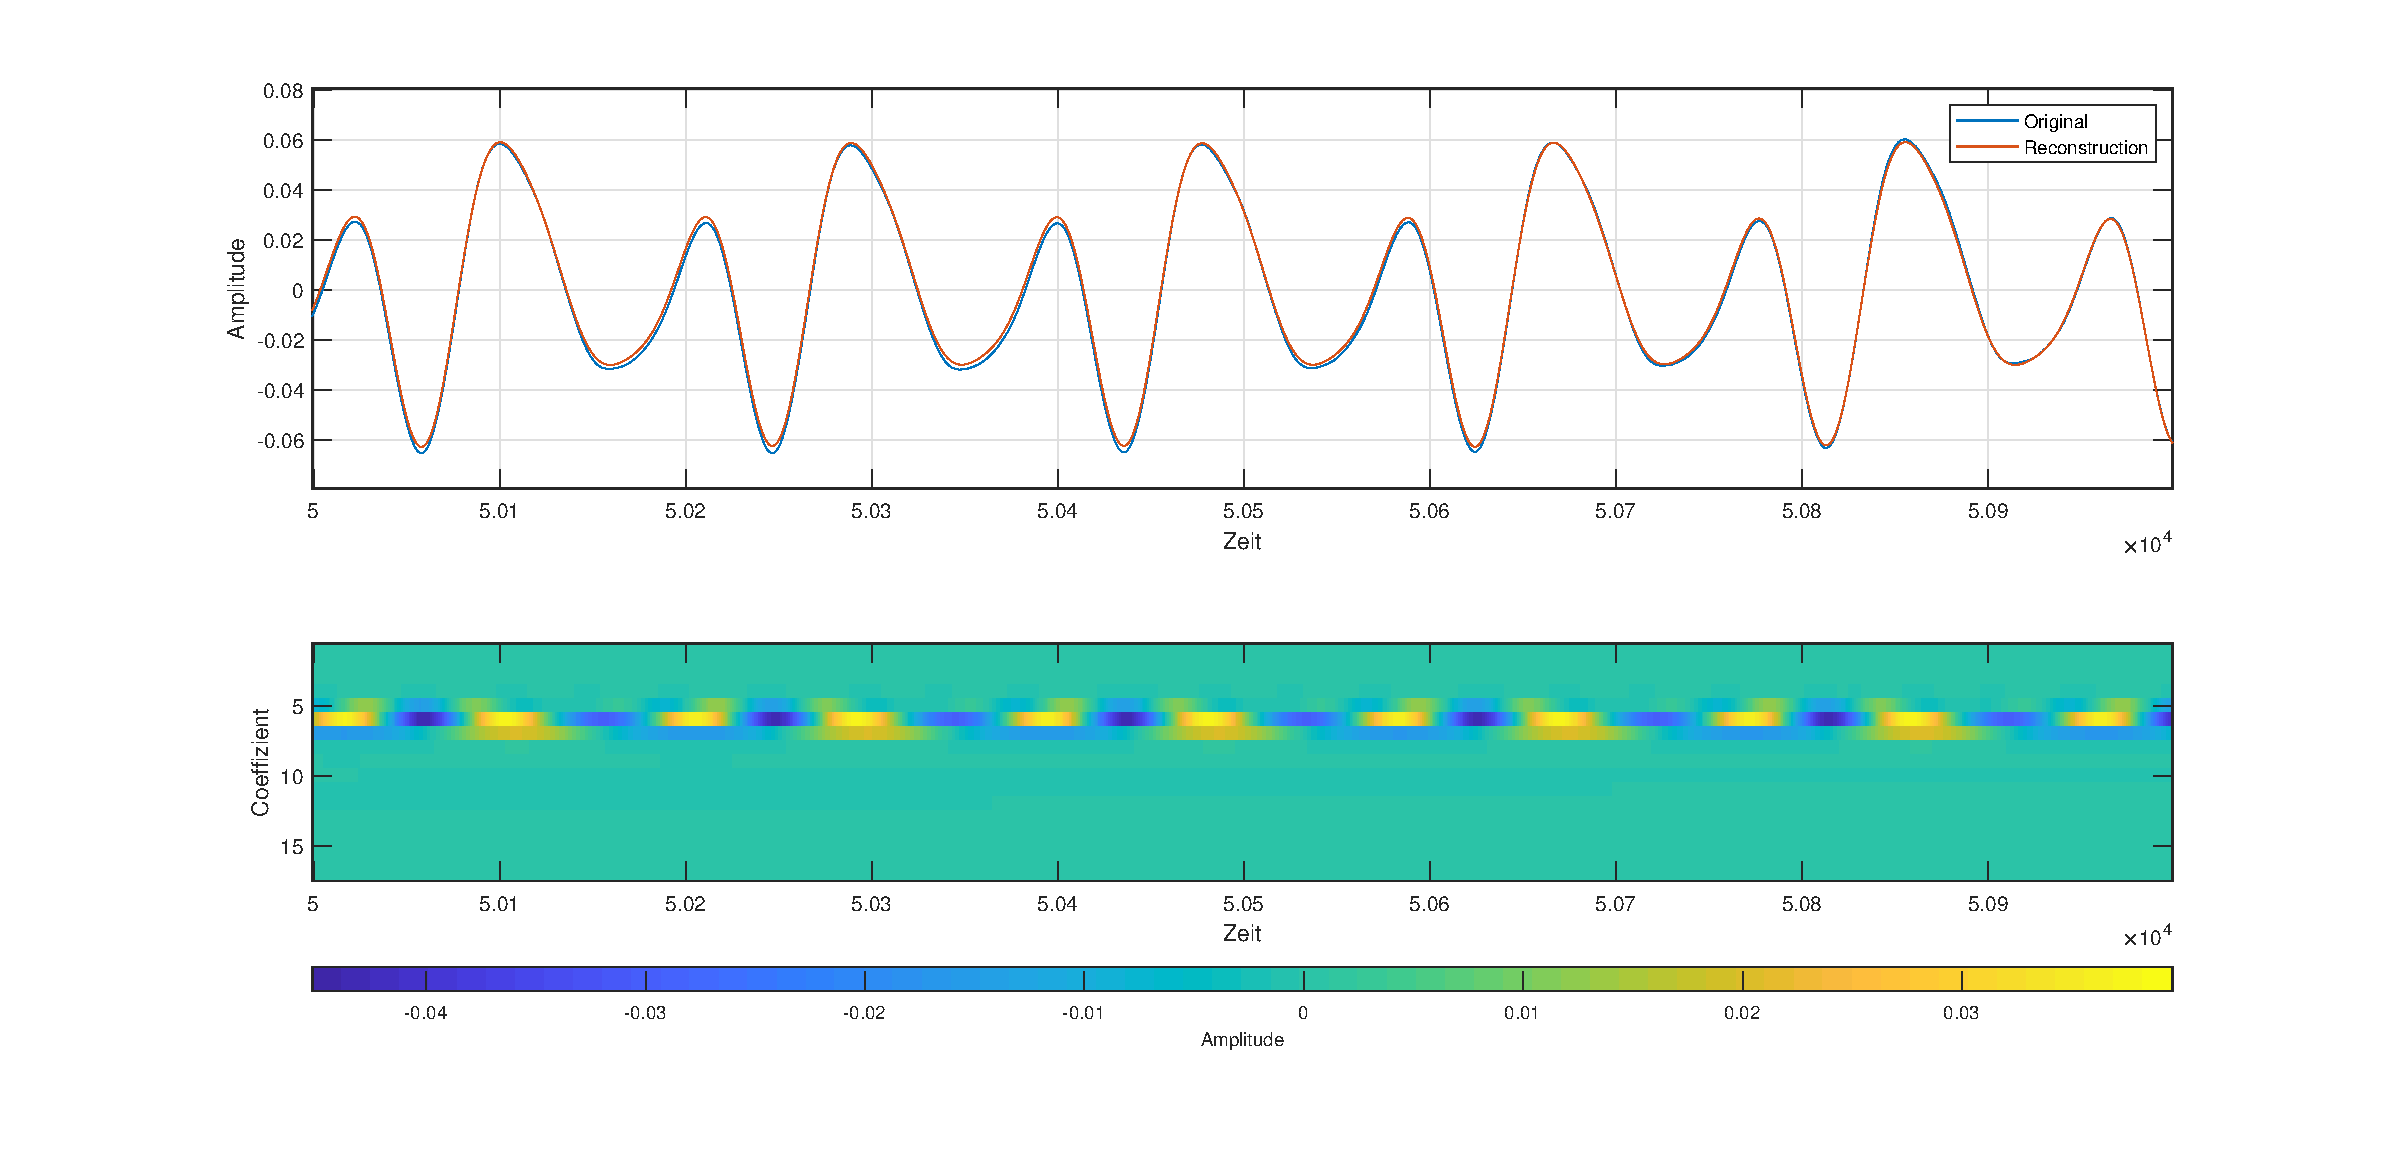
\includegraphics[width=\linewidth]{papers/compress/Bilder/frenchHorn_normal.pdf}
	\caption{Analyse eines Horntons mit dem Daubechies Wavelet db20.}
	\label{fig:horn}
\end{figure}

Als zweites Beispiel wird in \autoref{fig:horn} ein Horn-Ton untersucht.
Auch hier kann das harmonische Signal mit wenigen Koeffizienten recht exakt beschrieben werden. 
Zum Vergleich sind in \autoref{fig:dbHorn} die Anteile der Levels mit einem db4 und einem db20 abgebildet.
\begin{figure}
	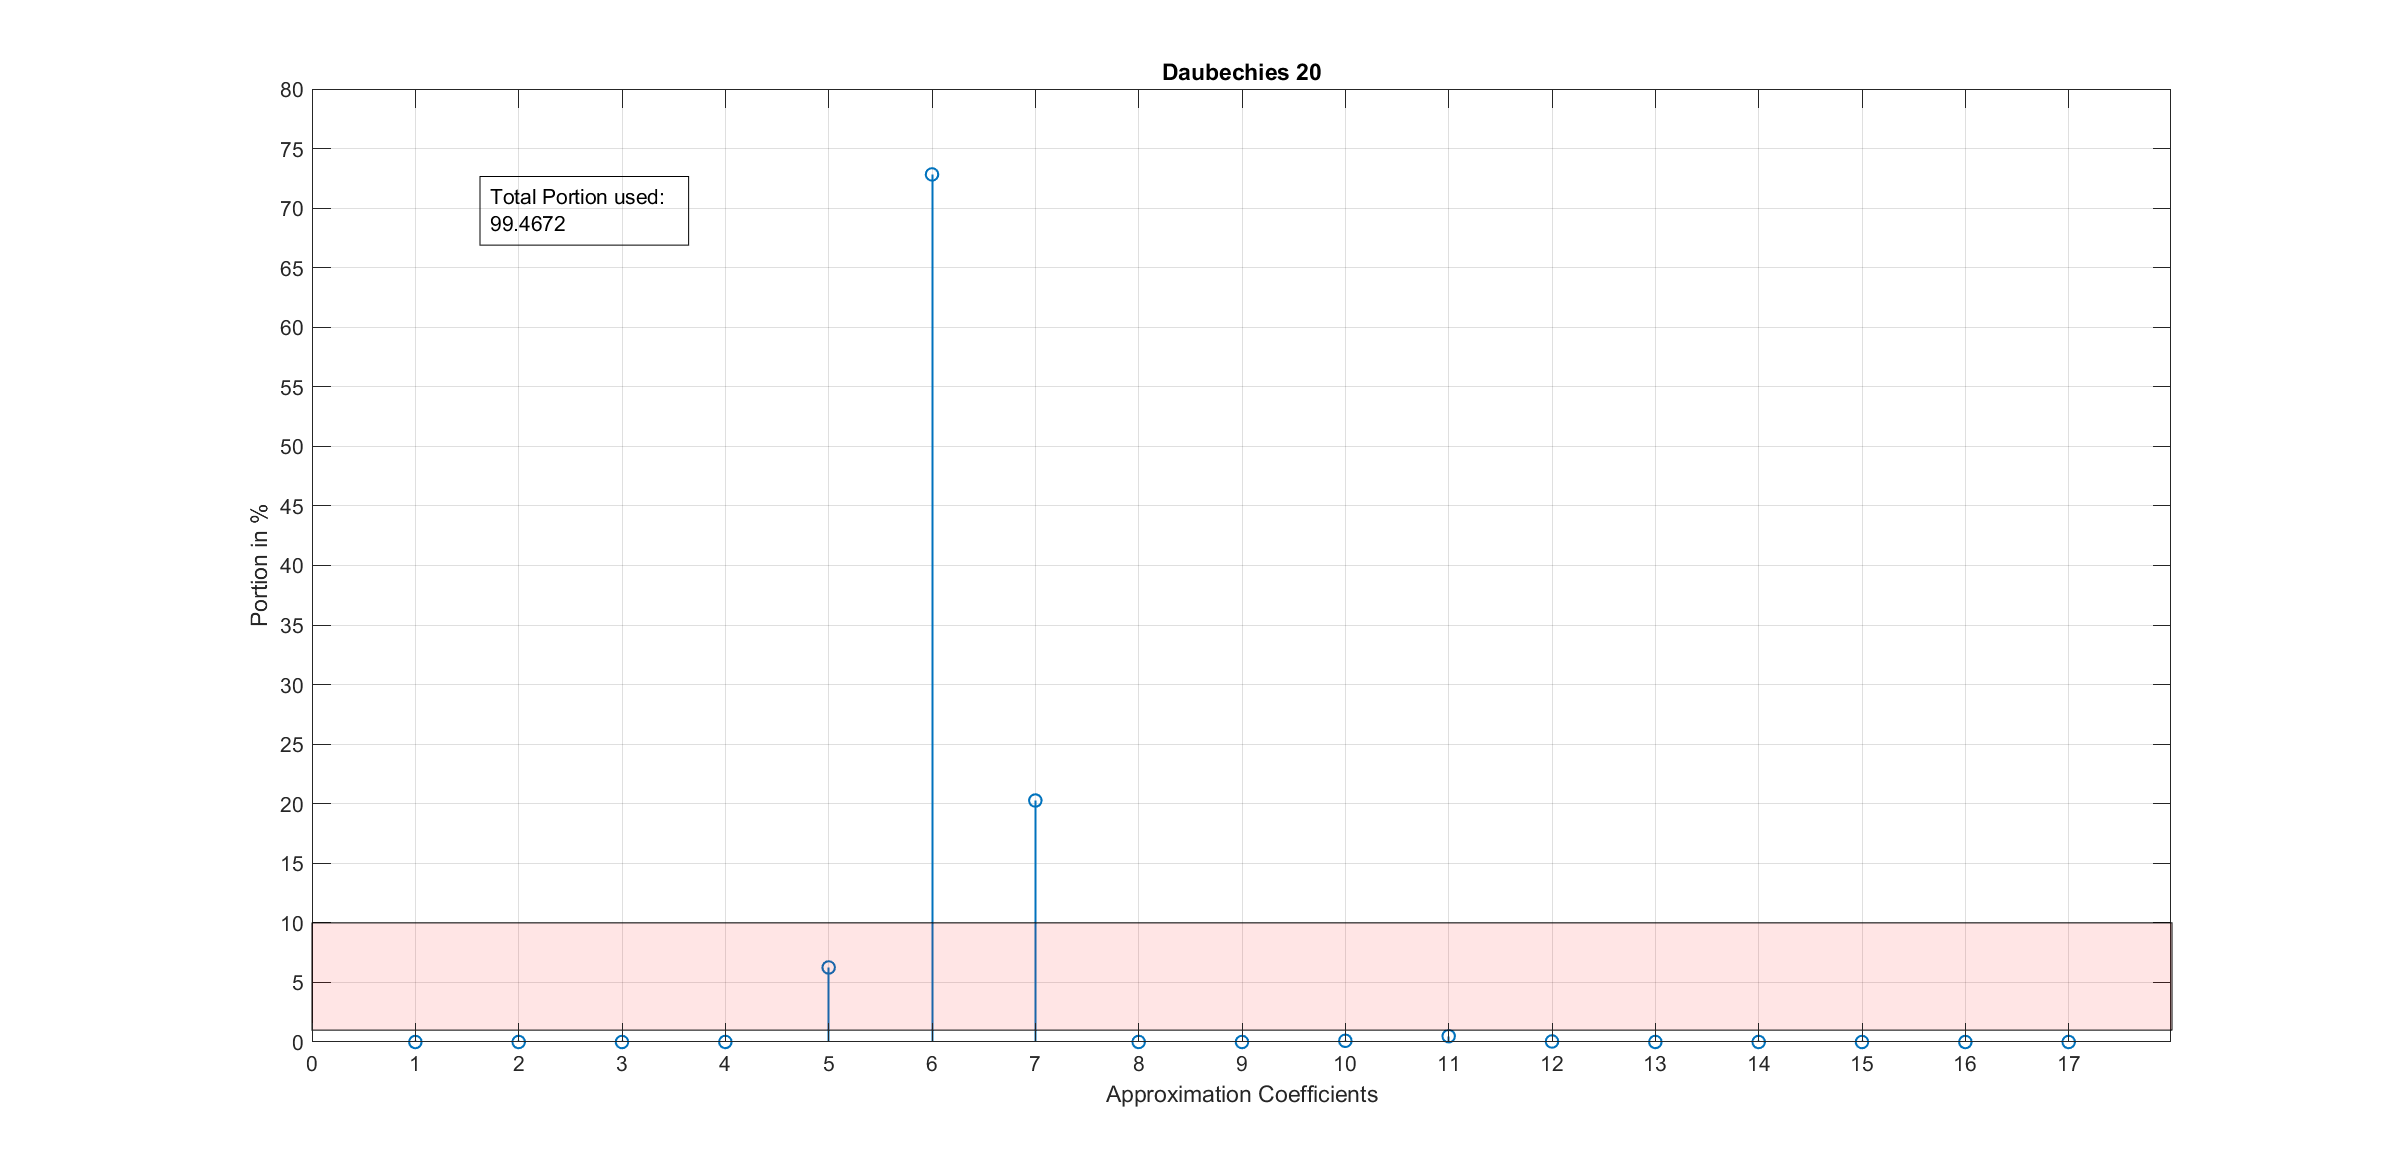
\includegraphics[width=0.5\linewidth]{papers/compress/Bilder/frenchHorn_db20.pdf}
	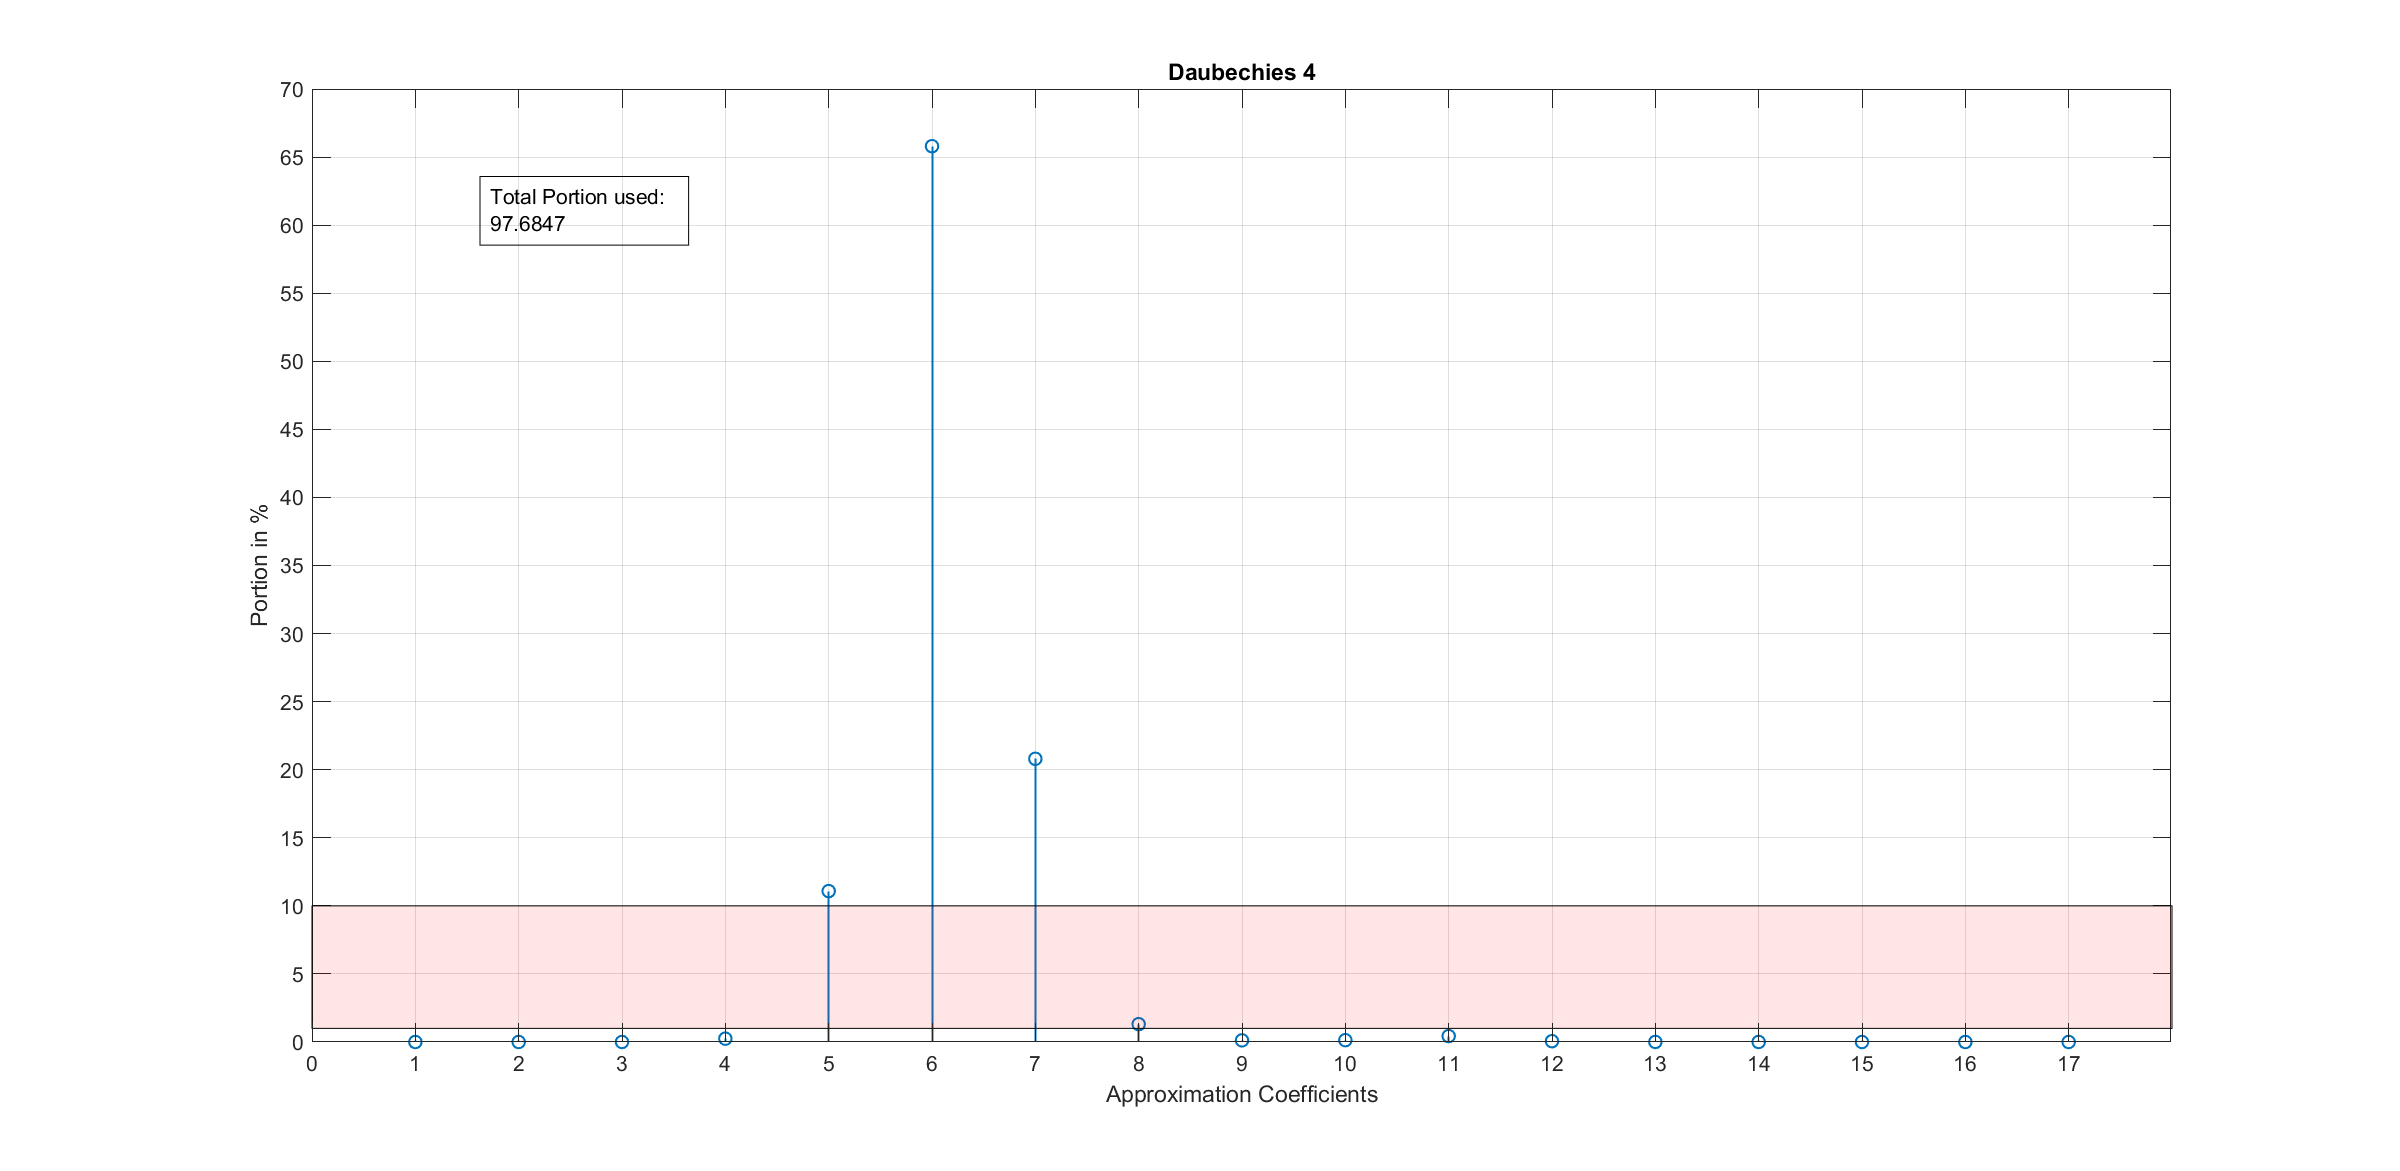
\includegraphics[width=0.5\linewidth]{papers/compress/Bilder/frenchHorn_db4.pdf}
	\caption{Anteil der verschiedenen Levels einer MSA an einem Hornton. Verwendet wurden Daubechies Wavelets der Ordnung vier und zwanzig.}
	\label{fig:dbHorn}
\end{figure}
Das Interessante ist nun, dass das harmonische Signal sehr gut mit dem db20 erfasst wird und über $99\,\text{\%}$ mit nur 3 Koeffizienten rekonstruiert werden kann.
Wird das Signal jedoch rekonstruiert zeigt sich ein grosses Problem der Quantisierung.
Das Signal wird teilweise stark verzerrt, was in \autoref{fig:hornRec} gut ersichtlich ist.
Obwohl diese Verzerrungen anteilsmässig keinen grossen Unterschied zum Originalsignal machen, sind diese hochfrequenten Störungen akustisch sehr gut wahrnehmbar.
Bei der Analyse mit dem db4 wird das Signal zwar weniger exakt rekonstruiert, jedoch werden keine Levels quantisiert.
Somit entstehen keine Verzerrungen und akustisch ist kaum ein Unterschied erkennbar.
\begin{figure}
	\centering
	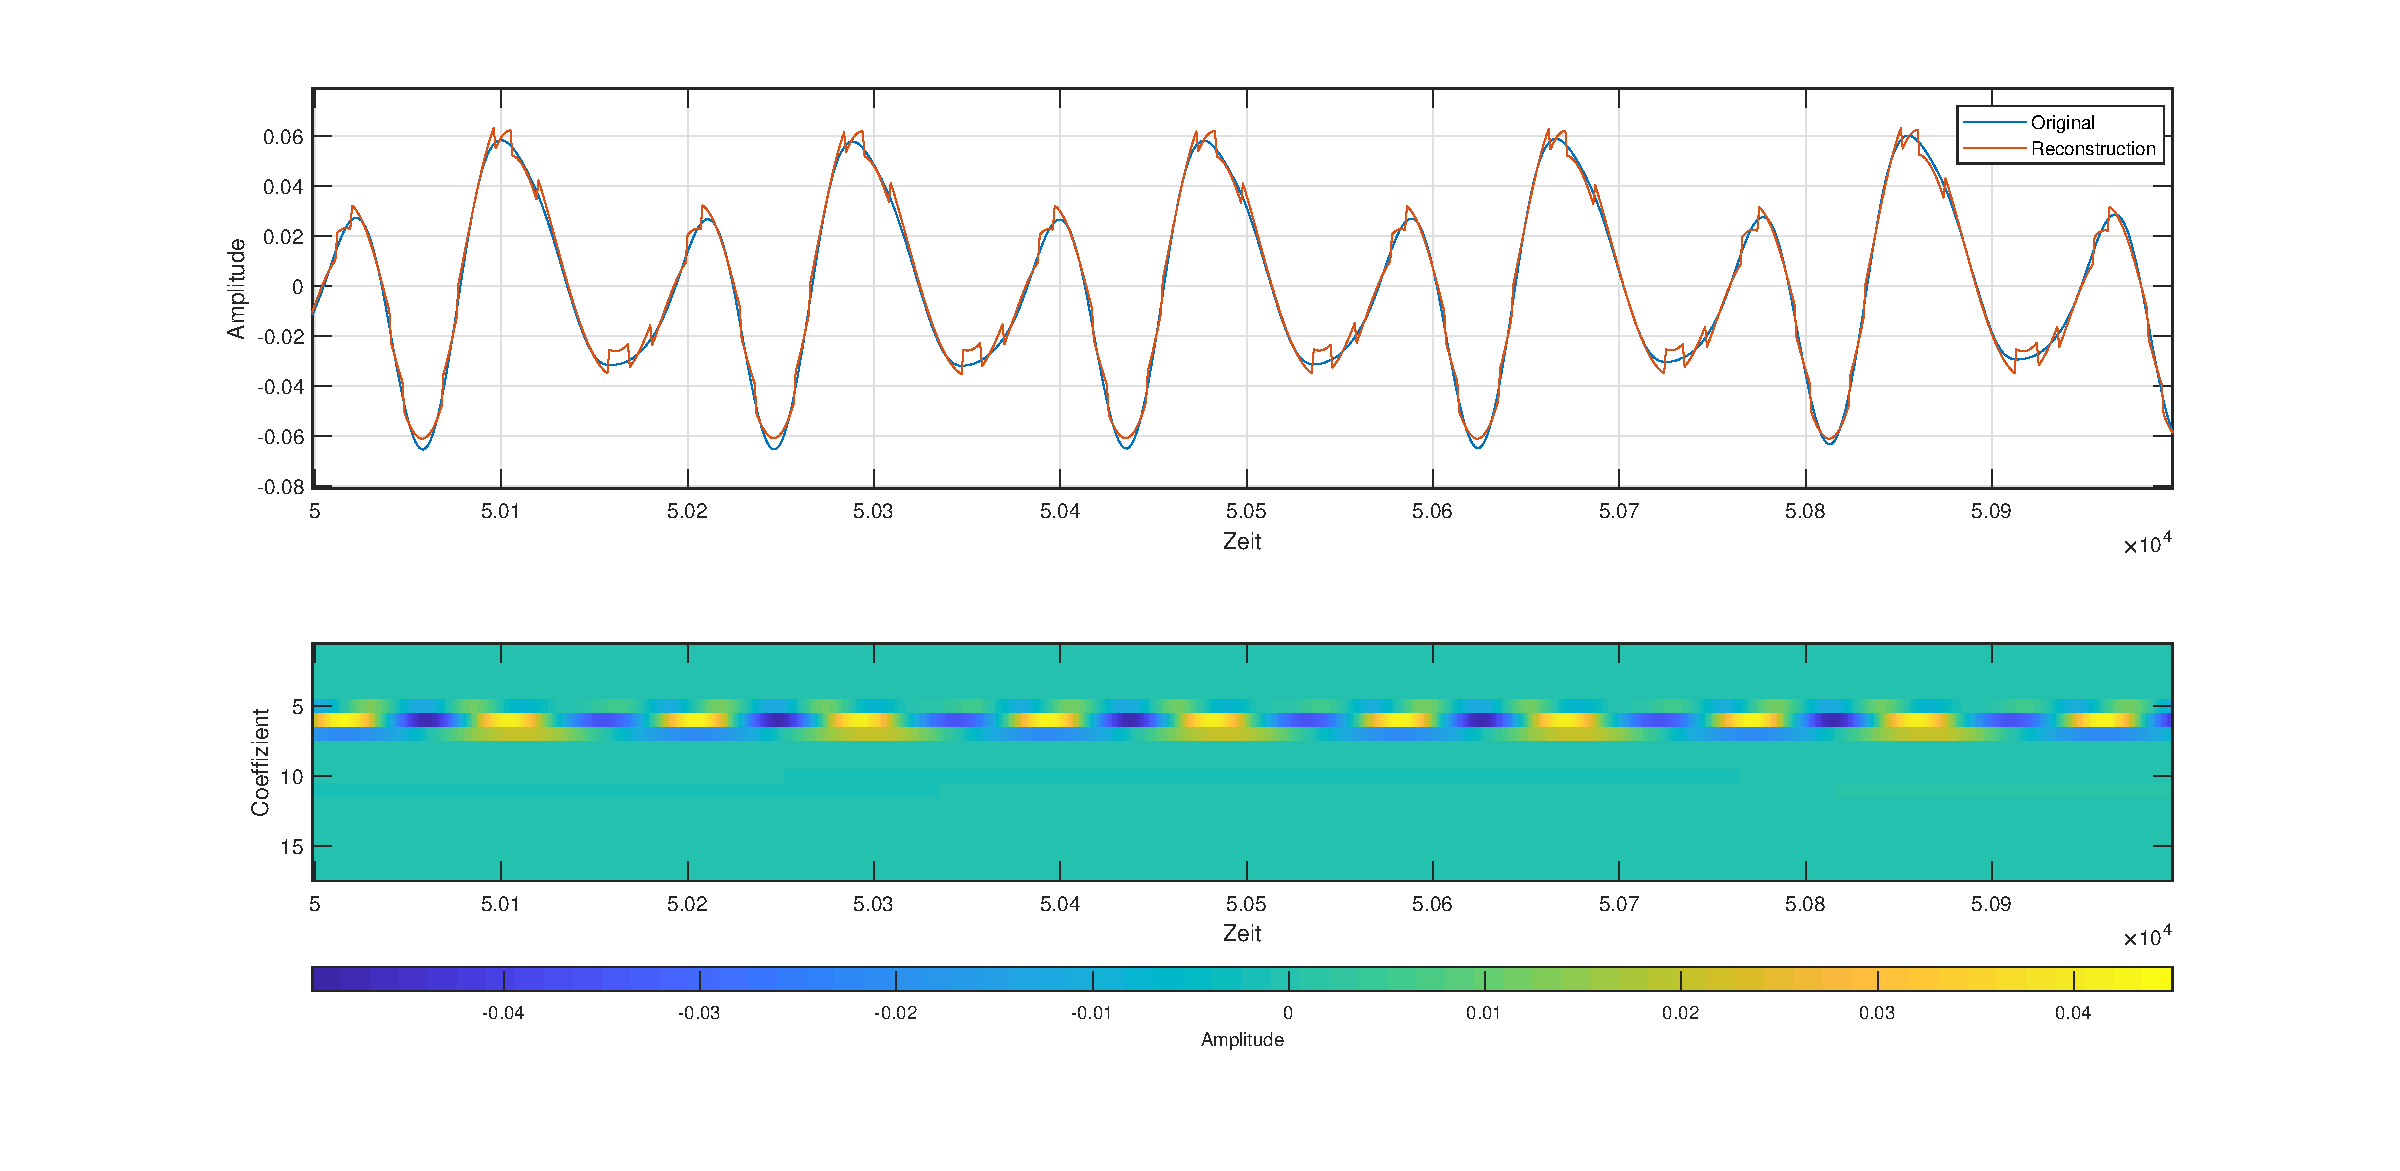
\includegraphics[width=\linewidth]{papers/compress/Bilder/frenchHorn_rec.pdf}
	\caption{Starke Verzerrungen des Horntons nach einer Rekonstruktion mit dem db20.}
	\label{fig:hornRec}
\end{figure}

\subsection{Transiente Signale}
Da im Audiobereich nicht nur harmonische Komponenten vorhanden sind soll diese Analyse auch auf transiente Signale angewendet werden.
Dabei soll auch wieder die Auswirkungen einer Quantisierung überprüft werden.
Als Signal wird der Ruf eines Vogels, dem Wendehals (\textit{Jynx torquilla}), verwendet.
Der Wendehals hat einen sehr charakterischen Ruf mit transienten Übergängen.
\begin{figure}
	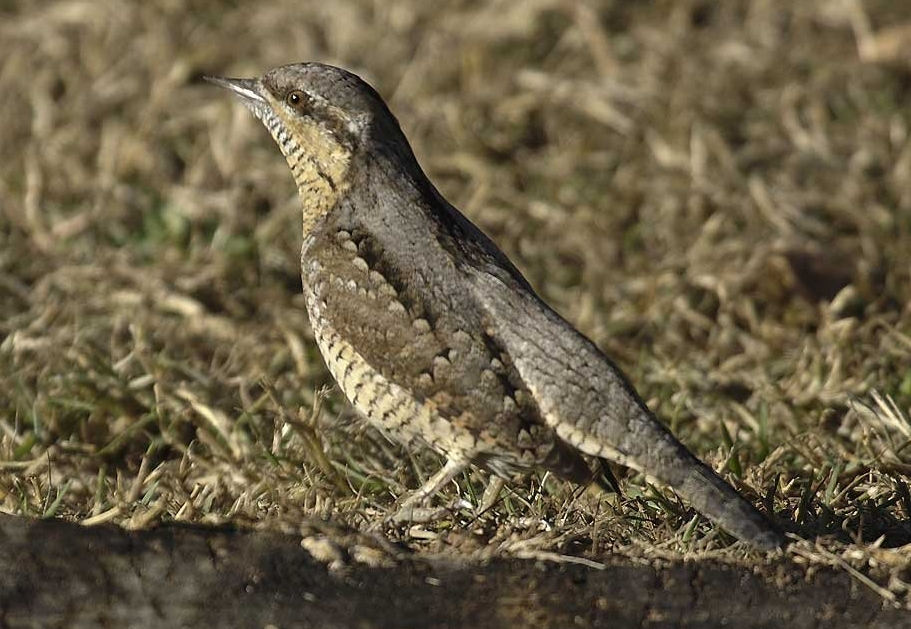
\includegraphics[width=0.4\linewidth]{papers/compress/Bilder/wendehals.jpg}
	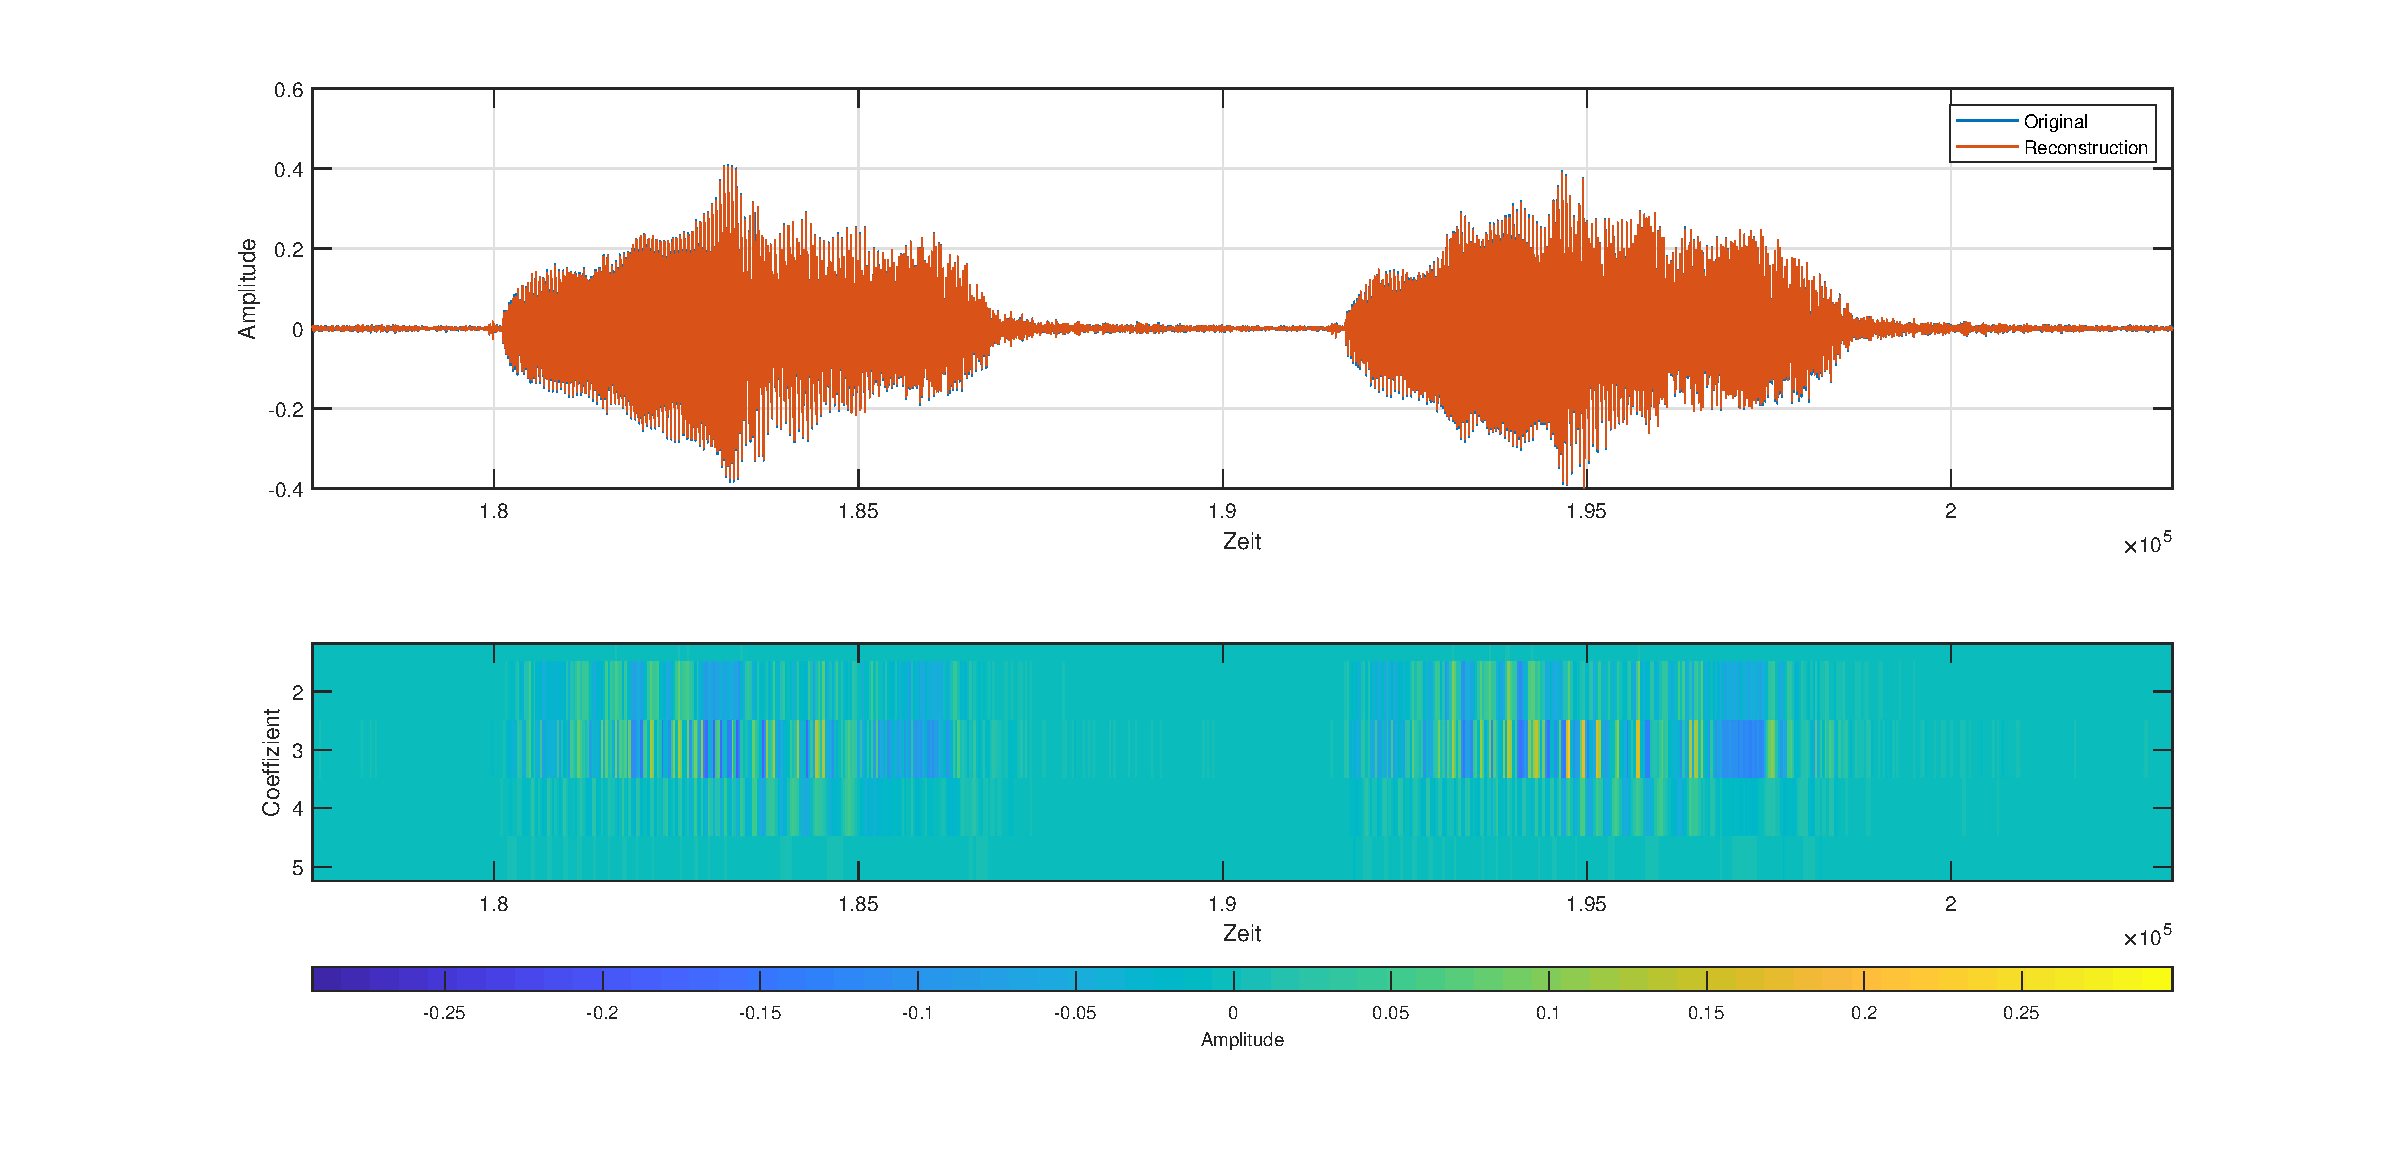
\includegraphics[width=0.6\linewidth]{papers/compress/Bilder/jynxAll.pdf}
	\caption{Der Wendehals (\textit{Jynx torquilla}) \cite{wikipedia:wendehals} mit seinem charakteristischen Ruf und der MSA.}
	\label{fig:jynxAll}
\end{figure}

Wie auch beim vorangehenden Beispiel ist der grösste Signalanteil in wenigen Koeffizienten der Multiskalenanalyse enthalten.
Durch die transienten Signale ist jedoch auch in den wichtigen Diletationslevels eine ausgeprägte Magnitude vorhanden.
In \autoref{chapter:daubechies} wurde erklärt, dass mit den Daubechies-Wavelets Signale von gleicher und auch höherer Ordnung, wie das Wavelet selber erkannt werden können. 
Experimentell hat sich gezeigt, dass mit höheren Wavelets eine bessere Rekonstruktion erreicht wird als mit den tiefen.
Das bedeutet aber nicht zwingend, dass die höheren Wavelets besser geeignet sind.
Jedoch sind bei den tieferen Diletationslevels die Wavelets breiter verteilt als bei den hohen und somit ist die Wahrscheinlichkeit grösser, dass ein Koeffizient quantisiert oder gelöscht wird. 
\begin{figure}
	\centering
	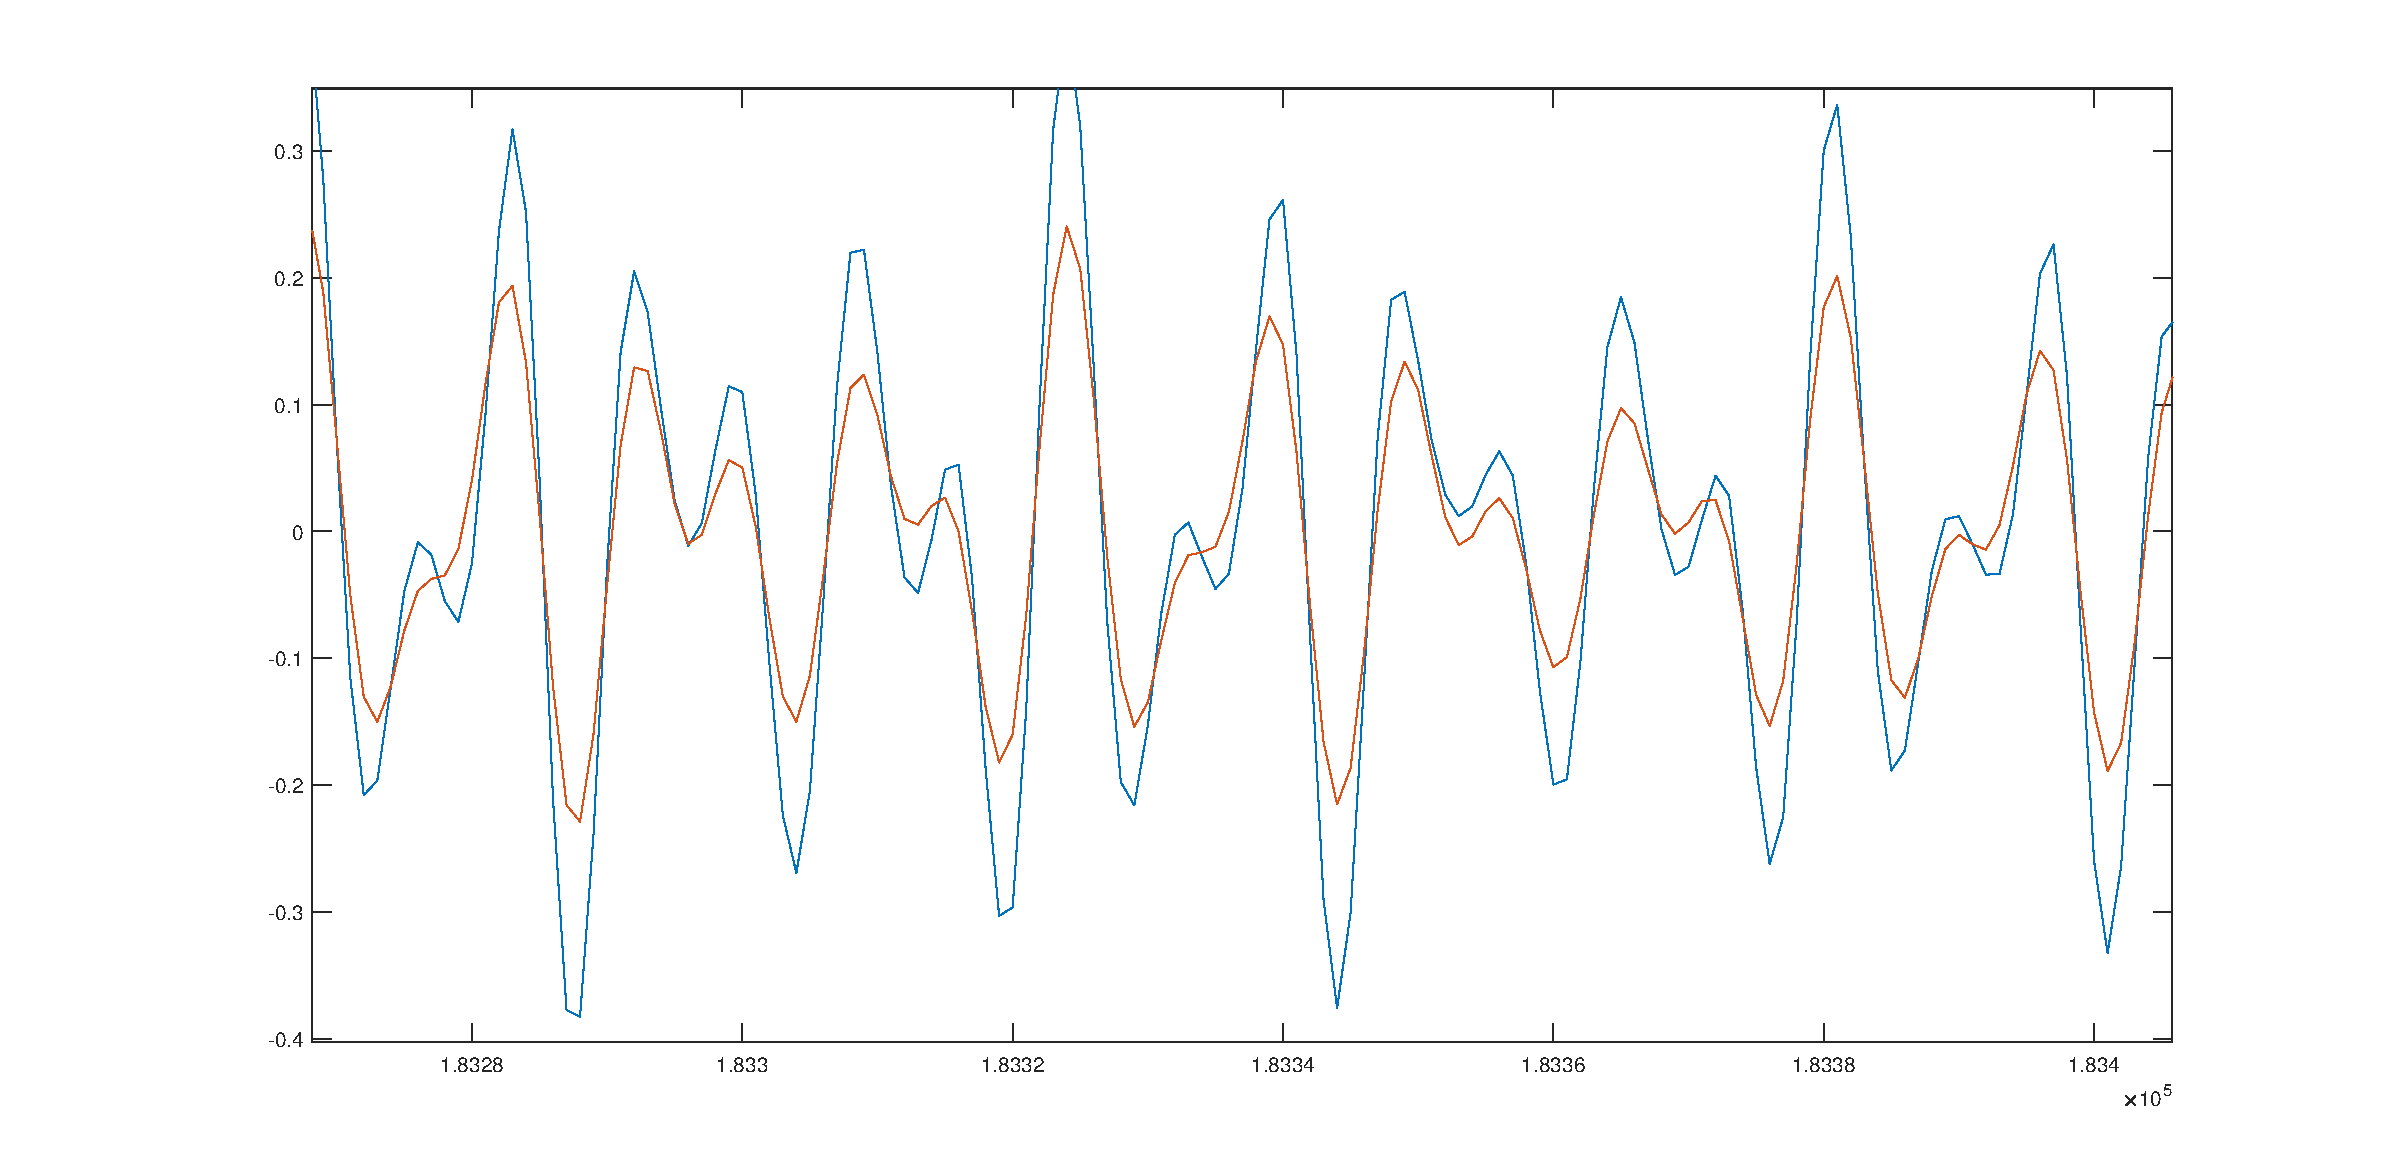
\includegraphics[width=\linewidth]{papers/compress/Bilder/jynxNear.pdf}
	\caption{Rekonstruktion des Vogelrufs, bei der nur das 6. Diletationslevel verwendet wurde, welches ungefährt $75\,\textbf{\%}$ des Signals enthält.}
	\label{fig:jynx6}
\end{figure}
Es ist besonders erstaunlich, dass mit einem db20 Wavelet fast $75\,\text{\%}$ des gesamten Signals nur im 6. Level vorhanden ist.
In \autoref{fig:jynx6} ist eine Rekonstruktion zu sehen, bei welcher ausschliesslich dieses Level verwendet wird.
Akustisch ist der Klang des Wendehals immernoch gut erkennbar, jedoch ist die Energie und somit die Lautstärke des Signals niedriger.

\section{Schlussfolgerung}
\rhead{Schlussfolgerung}
Das Ziel dieser Arbeit war es, Erkenntnisse zur Audiokomprimierung mit Wavelets zu erhalten.
Wie sich herausstellt, ist es mit relativ geringem Aufwand möglich, eine Multiskalenanalyse mit numerischen Programmen wie MATLAB durchzuführen.
Die Beispiele haben gezeigt, dass die Gruppierung in wichtige, unwichtige und zu quantisierende Koeffizienten zu grob gemacht wurde. 
Zum einen kann kaum für all die unterschiedlichen Signaltypen im Audiobereich die selbe Grenze verwendet werden. 
Zum anderen sollte diese Analyse auch auf der Zeitachse unterteilt werden und somit eine dynamischere Einteilung ermöglichen. 
Die Arbeit hat jedoch mit einfachen Beispielen gezeigt, dass sich Wavelets gut eignen, um solche Signale zu erfassen.
Harmonische und auch transiente Signale wurden beide mit wenigen Levels genau dargestellt.
Besondere Vorsicht soll der Quantisierung der Koeffizienten geboten werden, da sie bei gewissen Signale zu einer erheblichen verschlechterung des Hörerlebnis führen können.
In einem nächsten Schritt müsste von den erhaltenen Koeffizienten ausgehend ein passendes Audio-Format erstellt werden.

\printbibliography[heading=subbibliography]
\end{refsection}
